\documentclass[conference,a4paper]{IEEEtran}
\usepackage{cite}
\usepackage{etoolbox}
% Use colons rather than the default em dash after these headings.
\patchcmd{\abstract}{---\relax}{:\space\relax}{}{}
\patchcmd{\IEEEkeywords}{---\relax}{:\space\relax}{}{}
\usepackage{amsmath,amssymb}
\usepackage{graphicx}
\usepackage{booktabs}
\usepackage{tabularx}
\usepackage{array}
\usepackage[hidelinks]{hyperref}
\graphicspath{{figures/}}
\hyphenation{trans-crip-tomic re-pro-duc-ibil-ity}
\begin{document}
\title{Benchmarking Transcriptomic Feature Selection for Cross-Cohort Predictive Performance and Biomarker Reproducibility}
\author{\IEEEauthorblockN{Abbas El-Hajj Youssef \quad Jad Mcheik}
\IEEEauthorblockA{Department of Computer Science, American University of Beirut\\
Beirut, Lebanon\\
\href{mailto:aae145@mail.aub.edu}{aae145@mail.aub.edu} \quad
\href{mailto:jmm60@mail.aub.edu}{jmm60@mail.aub.edu}}}
\maketitle
\begin{abstract}
Predictive performance and reproducibility of selected genes are complementary objectives in transcriptomic biomarker research. We compared LASSO, Elastic Net, Stability Selection, StableMate and TENTACLES using 689 intestinal RNA-seq samples from four cohorts (495 Crohn's disease and 194 \emph{Not IBD}) and 9,983 common genes. In leave-one-cohort-out evaluation, panels selected on three cohorts were assessed on the fourth using an identical class-balanced logistic classifier. Predictive discrimination was evaluated alongside selected-gene overlap, differential-expression and random-panel baselines, and panel-size sensitivity. Mean held-out AUROC ranged from 0.628 for Stability Selection to 0.731 for Elastic Net (LASSO 0.728; TENTACLES 0.723), while TENTACLES attained the highest mean balanced accuracy (0.655). Simple training-only differential-expression panels were competitive: the top ten genes ranked by limma-voom and Welch's test yielded mean AUROCs of 0.748 and 0.772, respectively. TENTACLES produced the highest mean gene-set Jaccard across leave-one-cohort-out selections (0.210), compared with LASSO (0.102) and Elastic Net (0.092); however, the training cohorts overlap, and a size-matched uniform null does not account for that dependence. Independently fitted LASSO and Elastic Net panels showed substantially lower agreement. Results varied by cohort and panel size, with overlapping uncertainty intervals. Reactome analysis of TENTACLES panels identified enriched pathways in three of four cohorts, but the available comparison groups do not establish Crohn's-disease specificity. Cross-cohort predictive performance and gene-selection reproducibility should therefore be assessed separately and interpreted in light of cohort heterogeneity and model-selection constraints.
\end{abstract}
\begin{IEEEkeywords}
Crohn's disease, RNA sequencing, feature selection, cross-cohort validation, biomarker reproducibility
\end{IEEEkeywords}
\section{Introduction}
\label{sec:introduction}
Crohn's disease (CD) is a chronic inflammatory disorder of the gastrointestinal tract with substantial variation among patients \cite{torres2017crohn}. RNA sequencing (RNA-seq) measures RNA abundance in tissue samples and provides expression estimates for thousands of genes \cite{conesa2016survey}. Comparing intestinal expression profiles from patients with CD and comparison groups can reveal disease-associated patterns that may inform biomarker research \cite{montesi2026tentacles}. These associations do not, by themselves, establish causation or clinical usefulness.

Machine-learning classifiers can use expression measurements to distinguish CD from \emph{Not IBD} samples. Yet the number of genes typically exceeds the number of patients, and many genes are correlated. Feature selection therefore narrows the measurements to a \emph{gene signature}: a subset used for prediction or subsequent biological analysis. This creates two separate questions. \emph{Predictive generalisation} asks whether a model correctly classifies samples from a cohort excluded from training. \emph{Gene-signature reproducibility} asks whether fitting a comparable selection procedure separately to different patient cohorts yields similar gene lists. A model can generalise while selecting different genes from one dataset to another.

For example, two correlated genes may carry similar predictive information, so a selection method can retain either one depending on the patients analysed. Ein-Dor \emph{et al.} found markedly different yet similarly predictive signatures in breast cancer expression data \cite{eindor2005outcome}; related work showed that reliable agreement could require much larger discovery samples \cite{eindor2006thousands}. These studies motivate measuring gene agreement separately from prediction. Agreement is not proof of a causal biomarker, and its magnitude also depends on signature size.

Cohorts introduce further variation through differences in tissue composition, patient populations, sequencing protocols and class balance. Random train--test splits within one study can preserve such study-specific characteristics in both partitions. Cross-study evaluation instead tests models on cohorts not used for development \cite{bernau2014cross}. We use leave-one-cohort-out (LOCO) evaluation, training on three cohorts and testing on the fourth in turn.

Existing approaches differ in what they try to stabilise. LASSO selects genes through sparse regression coefficients \cite{tibshirani1996lasso}; Elastic Net also accommodates correlated predictors \cite{zou2005elastic}. Stability Selection favours genes repeatedly selected from subsamples \cite{meinshausen2010stability}, whereas StableMate targets predictors whose associations remain comparatively stable across environments \cite{deng2024stablemate}. TENTACLES combines feature-importance evidence from several learning algorithms into a consensus panel \cite{montesi2026tentacles}. Selection frequency, between-environment stability and agreement between algorithms are distinct properties; none alone guarantees replication across independent cohorts.

TENTACLES has already studied this Crohn's disease collection and compared biomarker-selection approaches \cite{montesi2026tentacles}. We instead examine how \emph{predictive transfer} relates to \emph{gene-set consistency} across LASSO, Elastic Net, Stability Selection, StableMate and TENTACLES, anchored against simple no-selection, univariate differential-expression and size-matched random-panel baselines. Our four analytical cohorts contain 689 samples from six BioProjects and share 9,983 genes. Alongside method-specific predictions, a fixed downstream classifier assesses all selected panels and baselines under identical prediction settings. We compare gene overlap against size-aware random-panel expectations, evaluate fixed-$K$ panel-size sensitivity, test sensitivity to source quality-control flags in D3, and review Reactome pathway agreement.

\section{Materials and Methods}
\subsection{Data sources and cohort characteristics}
\label{sec:dataset}
We used the processed intestinal tissue RNA-seq count matrices compiled for TENTACLES \cite{montesi2026tentacles}; we did not reprocess raw sequencing reads. The collection contains 689 samples labelled CD (495) or \emph{Not IBD} (194), grouped into four analytical cohorts from six BioProjects (Table~\ref{tab:cohorts}). The comparison label is retained from the source data, but does not imply that every control was a healthy volunteer. For instance, D3 includes non-tumour intestinal tissue from colorectal-cancer surgery \cite{friedrich2021il1}, and none of the four cohorts includes ulcerative colitis or non-IBD infectious colitis comparators.

\begin{table}[!t]
\caption{Cohort composition by source BioProject.}
\label{tab:cohorts}
\centering\footnotesize
\setlength{\tabcolsep}{3.5pt}
\renewcommand{\arraystretch}{1.1}
\begin{tabular}{@{}llrrr@{}}
\toprule
Cohort & BioProject(s) & $n$ & CD & Not IBD\\
\midrule
D1 & PRJNA248469 & 260 & 218 & 42\\
D2 & \shortstack[l]{PRJNA565216\\PRJNA985602} & 179 & 134 & 45\\
D3 & PRJNA702434 & 76 & 34 & 42\\
D4 & \shortstack[l]{PRJNA728646\\PRJNA961704} & 174 & 109 & 65\\
\midrule
Total & Six BioProjects & 689 & 495 & 194\\
\bottomrule
\end{tabular}
\end{table}

The CD fraction ranges from 44.7\% (D3) to 83.8\% (D1), and median assigned counts across common genes range from 1.78 to 12.01 million per sample. The cohorts also differ in tissue site: D1 comprises ileal biopsies; D2 includes ileal and colonic biopsies; D3 includes small- and large-intestinal samples; and D4 does not provide tissue-site labels in the supplied metadata. Source count CSVs lacked sample identifiers and had 670 rows ordered differently from their metadata. We recovered the IDs from accompanying R data files, aligned expression rows to metadata and checked count/label correspondence without altering the expression values.

The original matrices arrived with 10,061 genes for D1--D3 and 41,257 genes for D4; intersecting gene symbols without inspecting disease labels produced our 9,983-gene shared universe. Because raw FASTQ files were not re-quantified and exact upstream filtering logs for D1--D3 were not supplied in the published archive, all evaluated methods inherit this identical upstream input restriction. Its absolute impact on cross-cohort discrimination, potential degree of upstream leakage and possible differential effect across selectors cannot be established without upstream provenance or raw-read reprocessing.

Seven D3 records carried source exclusion flags (\texttt{qc=EXCLUDE}) from the original study's quality-control assessment \cite{friedrich2021il1} (four CD: \texttt{SAMN17945351}, \texttt{SAMN17945455}, \texttt{SAMN17947683}, \texttt{SAMN17947802}; three \emph{Not IBD}: \texttt{SAMN17947199}, \texttt{SAMN17947323}, \texttt{SAMN17947407}). Retaining all 76 D3 samples in the primary benchmark preserves exact alignment with Montesi \emph{et al.} \cite{montesi2026tentacles}; in addition, we conducted a held-out D3 test-only rescoring sensitivity analysis ($n=69$: 30 CD, 39 \emph{Not IBD}) without retraining D1, D2 or D4. Exploratory principal-component analysis (PCA) shows cohort-associated expression structure alongside disease labels (Fig.~\ref{fig:pca}). It does not establish whether cohort separation is technical or biological and was not used in model fitting.

\begin{figure}[!t]
\centering
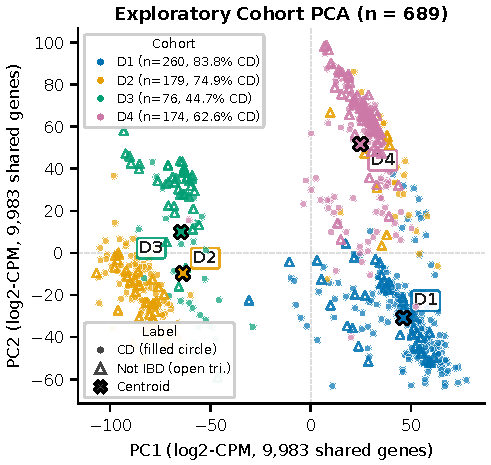
\includegraphics[width=\columnwidth]{cohort_pca_ieee.pdf}
\caption{Exploratory PCA of $\log_2(1+\mathrm{CPM})$ expression across 9,983 shared genes ($n=689$), encoded by cohort (colour), disease label (filled circle: CD; open triangle: \emph{Not IBD}) and cohort centroid ($\times$). This descriptive visualisation was not used in model fitting.}
\label{fig:pca}
\end{figure}

\subsection{LASSO and Elastic Net}
\label{sec:sparse_methods}
We used logistic-regression versions of LASSO and Elastic Net as sparse predictive baselines \cite{tibshirani1996lasso,zou2005elastic}. Both minimise a class-weighted logistic loss with a penalty on the gene coefficients $\boldsymbol{\beta}$ of the form
\begin{equation}
\Omega(\boldsymbol{\beta})=\alpha\lVert\boldsymbol{\beta}\rVert_1+
\frac{1-\alpha}{2}\lVert\boldsymbol{\beta}\rVert_2^2.
\label{eq:sparse_penalty}
\end{equation}
LASSO uses $\alpha=1$, whereas Elastic Net mixes $L_1$ and $L_2$ regularisation. The final LASSO models were fitted with \texttt{liblinear} coordinate descent \cite{fan2008liblinear}, using balanced class weights, tolerance $10^{-6}$ and inner-cross-validation selection over $C\in\{0.001,0.01,0.1,1\}$. Elastic Net was fitted with R \texttt{glmnet} \cite{friedman2010glmnet} at convergence threshold $10^{-12}$ followed by active-set Newton refinement. For both models, optimality was checked against Karush--Kuhn--Tucker conditions, including inactive coefficients and the intercept. Coefficients with absolute value greater than $10^{-8}$ defined the selected panel.

For each outer LOCO split, $(C,\alpha)$ was chosen by nested inner cross-validation within the three development cohorts using mean validation AUROC, with ties favouring stronger regularisation. Preprocessing (CPM $>1$ in at least 10\% of training samples, nonzero variance, $\log_2(1+\mathrm{CPM})$ and standardisation) was refitted strictly inside every training split; genes with $|\beta|>10^{-8}$ formed the selected signature. To evaluate gene agreement across patient-disjoint cohorts (zero shared samples), we also fitted LASSO and Elastic Net separately within each individual cohort using stratified inner cross-validation; their training-set predictions are not reported as external test results.

\subsection{Stability Selection}
\label{sec:stability_method}
We implemented complementary-pairs Stability Selection using a class-balanced $L_1$-logistic base model \cite{meinshausen2010stability}. Within each training set, 30 random partitions produced 60 complementary half-sample fits, with base regularisation calibrated on training data to select approximately 50 genes per fit. Each gene's selection frequency was its number of selections divided by 60. A frequency threshold of 0.75 resulted in one, zero, three and two selected genes in D1--D4, respectively. Since no classifier can be trained on the empty D2 panel, a threshold of $\pi \ge 0.60$ was chosen after observing these counts (four, nine, seven and five genes). This post-hoc change is explicitly disclosed, and fixed-$K$ analyses separately evaluate the complete selection-frequency ranking. The method-specific predictive pipeline (top-50 nonzero-frequency genes) is kept distinct from the $\pi \ge 0.60$ thresholded signature. This implementation computes complementary-pairs selection frequencies rather than using the authors' \texttt{stabs} package, and no theoretical false-selection bound is claimed.

\subsection{StableMate}
\label{sec:stablemate_method}
We used the authors' \texttt{StableMate} R package (version 0.1.0) \cite{deng2024stablemate}. For each LOCO fit, the three development cohorts defined the environments. The native procedure combined a random LASSO prefilter of 50 predictors per candidate, 2,000 candidate models in each of the prediction and stability ensembles, and 1,000 bootstrap replicates for importance estimation. A gene entered the stable-significant panel only if both its predictive and stability significance scores exceeded 0.975. Saved native StableMate predictions (four-cohort mean AUROC 0.743, balanced accuracy 0.624) were evaluated without repeating native training. In the separate controlled-classifier experiment, the fixed $L_2$ learner was refitted to the selected panel.

\subsection{TENTACLES consensus procedure}
\label{sec:tentacles_method}
We used the authors' \texttt{TENTACLES} R package (version 0.1.0) \cite{montesi2026tentacles} as an algorithm-consensus selector. On each LOCO development set, native RNA-seq preprocessing was followed by nine eligible classifier--selector pairs: random forest/correlation, MLP/ROC, bagged MLP/ROC, linear SVM/Boruta, C5 rules/Boruta, LightGBM/ROC, decision tree/Boruta, MARS/Boruta and PLS/Boruta, tuned with five-fold cross-validation, five candidate settings, class downsampling and F1 as target metric.

In the implementation used here, \emph{CD} was explicitly set as the positive class for cross-validation and F1-based tuning. The XGBoost/base component was omitted from consensus aggregation because complete feature-importance output was unavailable for every cohort, leaving nine eligible learners. A gene was retained when it received votes from at least six of these nine learners. A five-of-nine threshold was evaluated separately as a sensitivity analysis; it does not denote a different feature-selection algorithm. All feature selection was restricted to the development cohorts, and the common downstream logistic classifier provided the reported external predictions.

\subsection{Reference baselines}
\label{sec:baselines}
To anchor selector performance under the identical LOCO splits and controlled downstream classifier, we included four reference baselines fitted strictly within each training split over the shared 9,983-gene universe: (i) all 9,983 shared genes (no-selection baseline); (ii) all fold-specific training-eligible genes (CPM $>1$ in $\ge 10\%$ of training samples; 8,337--8,438 genes); (iii) training-only univariate differential expression (DE) via \texttt{limma-voom} \cite{law2014voom} (\texttt{\textasciitilde 0 + class + cohort} with \texttt{edgeR} TMM normalisation \cite{robinson2010edger}) and a Welch $t$-test companion (alphabetical gene-name tie-break) at $K\in\{10,25,50,100,200\}$; and (iv) size-matched random panels ($B=100$ draws per method-fold from each fold's training-eligible universe; 2,000 draws total). Within-cohort descriptive empirical $p$-values, $p_{\mathrm{emp}}=(1+\sum_{b=1}^{100}\mathbb{I}[m_b \ge m_{\mathrm{obs}}])/101$ (minimum resolution $1/101 \approx 0.0099$), benchmark panel-size-conditioned performance within each cohort and are not cross-method significance tests.

\begin{table}[!t]
\caption{Selected-gene panels evaluated by the controlled downstream classifier.}
\label{tab:method_overview}
\centering\footnotesize
\setlength{\tabcolsep}{3pt}
\renewcommand{\arraystretch}{1.12}
\begin{tabular}{@{}p{2.2cm}p{5.7cm}@{}}
\toprule
Method & Panel definition \\
\midrule
LASSO & Nonzero \texttt{liblinear} coefficients ($|\beta|>10^{-8}$, \texttt{tol=1e-6}) \\
Elastic Net & Nonzero \texttt{glmnet}+Newton coefficients ($|\beta|>10^{-8}$) \\
Stability Selection & Frequency $\geq 0.60$ (post-hoc fallback from $0.75$) \\
StableMate & Predictive and stability significance each $>0.975$ \\
TENTACLES & Consensus $\ge 6/9$ eligible voters (CD-positive orientation) \\
\bottomrule
\end{tabular}
\end{table}

\subsection{Cross-cohort evaluation and controlled classifier}
\label{sec:evaluation_design}
Each LOCO round held out one analytical cohort and used the other three for model development (Table~\ref{tab:splits}). Training and held-out samples were disjoint within each round. Because some cohorts comprise multiple BioProjects, this is cohort-level rather than six-study-level validation. In every training fold, gene eligibility filtering (CPM $>1$ in at least 10\% of training samples), $\log_2(1+\mathrm{CPM})$ transformation and z-score standardisation were fitted strictly on training samples and applied read-only to the held-out cohort, yielding eligible universes of 8,337 (D1), 8,406 (D2), 8,409 (D3) and 8,438 (D4) genes (four-way intersection: 8,237; disjoint single-cohort common intersection: 7,928).

\begin{table}[!t]
\caption{Outer LOCO assignments. Each held-out cohort is excluded from its own preprocessing, gene selection and model training.}
\label{tab:splits}
\centering\footnotesize
\begin{tabular}{@{}lrrl@{}}
\toprule
Test cohort & Train $n$ & Test $n$ & Development cohorts\\
\midrule
D1 & 429 & 260 & D2, D3, D4\\
D2 & 510 & 179 & D1, D3, D4\\
D3 & 613 & 76 & D1, D2, D4\\
D4 & 515 & 174 & D1, D2, D3\\
\bottomrule
\end{tabular}
\end{table}

To compare selected gene panels and reference baselines under an identical downstream learner, each panel selected from the development cohorts was evaluated with a fixed class-balanced $L_2$-regularised logistic regression (\texttt{scikit-learn} \cite{pedregosa2011scikit}, \texttt{liblinear}, $C=1.0$, seed 123, CD positive, probability threshold 0.5). Method-specific native predictions were retained separately and are not conflated with controlled-classifier scores.

\subsection{Prediction metrics and uncertainty}
\label{sec:predictive_metrics}
We report eight held-out metrics per cohort (AUROC, AUPRC, balanced accuracy, sensitivity, specificity, precision, F1 and Brier score) together with standardised 2,000-resample patient-stratified bootstrap 95\% confidence intervals for within-cohort AUROC and balanced accuracy across all five primary methods and reference baselines. Four-cohort means and sample standard deviations ($n-1$ denominator) are strictly descriptive; we do not perform pooled cross-fold hypothesis tests because the four LOCO folds share two-thirds of their training cohorts.

\subsection{Chance-adjusted gene overlap, fixed-$K$ sensitivity and pathway agreement}
\label{sec:reproducibility_metrics}
Let $S_{m,f}$ denote the genes selected by method $m$ when cohort $f$ is held out. Pairwise Jaccard similarity was averaged across all six unordered LOCO pairs:
\begin{equation}
\bar{J}_m=\frac{1}{6}\sum_{a<b}\frac{|S_{m,a}\cap S_{m,b}|}{|S_{m,a}\cup S_{m,b}|}.
\label{eq:jaccard}
\end{equation}
Because raw Jaccard scales with panel size and each fold has a distinct eligible universe $U_a \neq U_b$, we derived exact uniform-draw expected pairwise and four-way intersections:
\begin{align}
\mathbb{E}[|A \cap B|] &= \frac{k_a \, k_b \, |U_a \cap U_b|}{|U_a| \, |U_b|}, \label{eq:overlap_null_pw}\\
\mathbb{E}\!\left[\left|\bigcap_{i=1}^{4} A_i\right|\right] &= \left|\bigcap_{i=1}^{4} U_i\right| \prod_{i=1}^{4} \frac{k_i}{|U_i|}, \label{eq:overlap_null_4w}
\end{align}
paired with 10,000 independent uniform Monte Carlo draws per comparison to obtain 95\% null intervals for Jaccard similarity and the overlap coefficient. Because LOCO training folds share two of three cohorts, these uniform nulls provide a size-only chance reference rather than a dependence-calibrated hypothesis test.

To evaluate sensitivity to unequal panel sizes, we tested fixed panel sizes $K\in\{10,25,50,100,200\}$ strictly for continuously ranked methods: Stability Selection (ranked frequency; 4/4 folds across all $K$) and sparse $|\beta|$-ranked LASSO and Elastic Net strictly where $K \le n_{\mathrm{nonzero}}$ (otherwise flagged inapplicable). Unranked consensus sets (TENTACLES and StableMate) were excluded by design (0/4 evaluable folds) rather than forcing arbitrary tie-breaks; we report the number of evaluable folds for every panel size and do not equate partial-support averages ($1/4$ or $3/4$) with full four-fold averages.

For pathway agreement, Reactome v98 pathways \cite{ragueneau2026reactome} containing 10--500 eligible genes were tested for over-representation via one-sided hypergeometric tests with Benjamini--Hochberg correction ($q<0.05$) \cite{benjamini1995fdr}; pathway Jaccard was undefined when both sets were empty. Pathway findings are reported only for the gene panels evaluated with the final methods. Reactome enrichment was available for TENTACLES, Stability Selection and StableMate; enrichment of the final LASSO and Elastic Net panels was not performed.

\section{Results}
\label{sec:results}
\subsection{Prediction on excluded cohorts and reference baselines}
\label{sec:results_prediction}
Under the controlled $L_2$ logistic classifier, four-cohort mean AUROC across the five primary selectors ranged from 0.628 (Stability Selection, $\pi \ge 0.60$) to 0.731 (Elastic Net), with LASSO at 0.728 and TENTACLES at 0.723; mean balanced accuracy ranged from 0.563 to 0.655, highest for TENTACLES, which also achieved the highest mean AUPRC (0.843), F1 (0.704) and lowest Brier score (0.236) (Table~\ref{tab:results_main}; complete per-cohort eight-metric table with 2,000-resample 95\% bootstrap CIs in Table~\ref{tab:s1}). Method-native predictors differed notably in some cases (for example, native StableMate achieved mean AUROC 0.743 and balanced accuracy 0.624 versus 0.659 and 0.598 under the controlled classifier), illustrating why separating feature selection from downstream classification clarifies method comparisons.

\begin{table*}[!t]
\caption{Controlled five-method benchmark and reference baselines under identical class-balanced $L_2$ logistic regression ($C=1$; CD positive). AUROC and BA (balanced accuracy) are unweighted four-cohort means with sample SD ($n-1$ denominator). LOCO mean pairwise Jaccard ($\bar{J}$) averages six dependent fold pairs; Monte Carlo (MC) nulls are size-only chance references (10,000 draws), not dependence-calibrated hypothesis tests.}
\label{tab:results_main}
\centering\scriptsize
\resizebox{\textwidth}{!}{\begin{tabular}{@{}llrrrrrrrl@{}}
\toprule
Selector / Baseline & Role & Panel mean [min--max] & AUROC (SD) & BA (SD) & AUPRC & F1 & Brier & LOCO $\bar{J}$ (Obs / MC Null) & All 4\\
\midrule
Elastic Net & Primary & 124.3 [11--430] & 0.731 (0.103) & 0.583 (0.063) & 0.812 & 0.633 & 0.313 & 0.092 / 0.002 (49.1$\times$) & 0\\
LASSO & Primary & 120.0 [77--219] & 0.728 (0.067) & 0.620 (0.023) & 0.825 & 0.697 & 0.310 & 0.102 / 0.006 (16.2$\times$) & 2\\
TENTACLES & Primary & 76.5 [61--91] & 0.723 (0.100) & \textbf{0.655} (0.093) & \textbf{0.843} & \textbf{0.704} & \textbf{0.236} & \textbf{0.210} / 0.005 (46.3$\times$) & 6\\
StableMate & Primary & 15.8 [14--20] & 0.659 (0.083) & 0.598 (0.110) & 0.801 & 0.642 & 0.310 & 0.033 / 0.001 (34.9$\times$) & 0\\
Stability Selection\ ($\pi\ge 0.60$) & Primary & 6.3 [4--9] & 0.628 (0.051) & 0.563 (0.050) & 0.797 & 0.656 & 0.258 & 0.128 / 0.0004 (338.2$\times$) & 0\\
\midrule
All-9,983 Shared Genes & Baseline & 9,983 (all) & 0.681 (0.073) & 0.572 (0.035) & 0.775 & 0.659 & 0.336 & --- & ---\\
Train-Eligible ($\ge 10\%$) & Baseline & 8,397.5 [8,337--8,438] & 0.673 (0.130) & 0.592 (0.076) & 0.764 & 0.624 & 0.371 & --- & ---\\
\texttt{limma-voom} Top-10 & Baseline & 10 (fixed) & 0.748 (0.101) & 0.631 (0.094) & 0.856 & 0.723 & 0.215 & --- & ---\\
\texttt{limma-voom} Top-100 & Baseline & 100 (fixed) & 0.710 (0.117) & 0.649 (0.106) & 0.814 & 0.705 & 0.236 & --- & ---\\
Welch $t$-test Top-10 & Baseline & 10 (fixed) & 0.772 (0.081) & 0.601 (0.081) & 0.867 & 0.625 & 0.254 & --- & ---\\
Welch $t$-test Top-100 & Baseline & 100 (fixed) & 0.732 (0.083) & 0.660 (0.064) & 0.842 & 0.722 & 0.228 & --- & ---\\
\bottomrule
\end{tabular}}
\end{table*}

\begin{figure*}[!t]
\centering
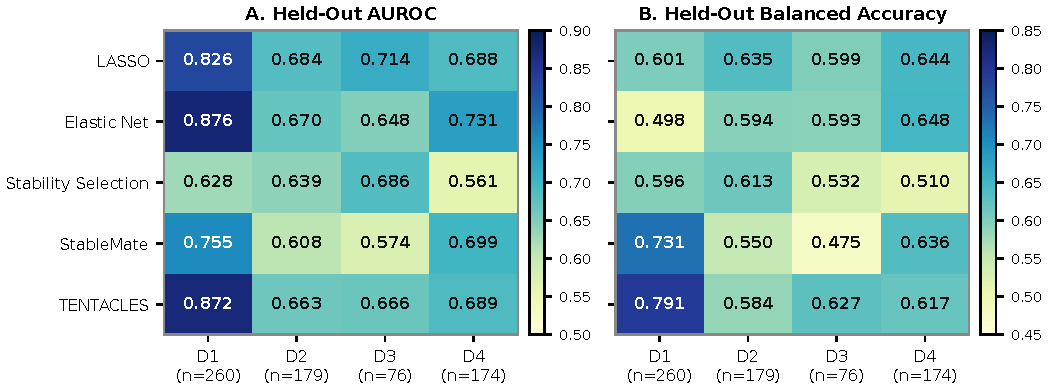
\includegraphics[width=\textwidth]{heldout_metric_heatmaps.pdf}
\caption{External test performance of all five feature-selection methods, separately for each left-out cohort under the identical fixed class-balanced $L_2$ logistic classifier ($C=1$). Entries show (A) AUROC and (B) balanced accuracy at probability threshold 0.5. Cohort sample counts are given below D1--D4; darker cells indicate higher values.}
\label{fig:results_heatmap}
\end{figure*}

Performance depended strongly on the held-out cohort, and within-cohort 95\% bootstrap CIs overlapped substantially across methods (Fig.~\ref{fig:results_heatmap} and Fig.~\ref{fig:tradeoff}B). On D1, Elastic Net (0.876 [0.831, 0.918]) and TENTACLES (0.872 [0.819, 0.916]) attained the highest AUROCs, whereas Stability Selection obtained 0.628 [0.531, 0.717]. On D2 and D3, LASSO led (0.684 and 0.714); on D4, Elastic Net led (0.731). While D1 and D4 occupy positive PC1 coordinates in Fig.~\ref{fig:pca}, this visual proximity is strictly an exploratory observation rather than a causal explanation for D1 performance, as D1 also has the highest CD prevalence (83.8\%) and uniform ileal biopsies.

Reference baselines under the identical classifier provided an essential anchor (Table~\ref{tab:results_main}; Tables~\ref{tab:s2}--\ref{tab:s3}). All-9,983 shared genes achieved mean AUROC 0.681 (SD 0.073; BA 0.572) and Train-Eligible ($\ge 10\%$) achieved 0.673 (sample SD 0.130; BA 0.592). Training-only univariate differential expression achieved competitive discrimination across the entire $K\in\{10,25,50,100,200\}$ curve (\texttt{limma-voom}: 0.748 at $K=10$ to 0.710 at $K=100$; Welch: 0.772 at $K=10$ to 0.732 at $K=100$; reported descriptively without post-hoc selection of a single best $K$). Size-matched random panels ($B=100$) attained strong baseline AUROCs on D1 (mean 0.794--0.796 for $K=73$--$94$) and D4 (0.681--0.685), with only a minority of the 20 method-cohort cells falling below descriptive $p_{\mathrm{emp}} < 0.05$ (for example, Elastic Net on D1 at $K=11$, $p_{\mathrm{emp}}=0.0099$; TENTACLES on D1 BA, $p_{\mathrm{emp}}=0.0396$).

\subsection{TENTACLES consensus-vote sensitivity}
\label{sec:results_tentacles}
The TENTACLES six-of-nine consensus produced panels of 73, 91, 81 and 61 genes (D1--D4). The primary rule gave mean AUROC 0.723 and mean balanced accuracy 0.655. Relaxing the consensus to five votes selected 90--115 genes per fold and reduced mean AUROC to 0.691 (Table~\ref{tab:tentacles_sensitivity}). Six votes scored higher on D1, D3 and D4, but not on D2; it should not be described as uniformly superior.

\begin{table}[!t]
\caption{TENTACLES on each held-out cohort: prespecified 6/9-vote primary versus 5/9-vote sensitivity. AUROC intervals are 95\% patient-stratified bootstrap intervals (2,000 resamples), conditional on the fitted six-vote model.}
\label{tab:tentacles_sensitivity}
\centering\footnotesize
\setlength{\tabcolsep}{2.9pt}
\renewcommand{\arraystretch}{1.1}
\begin{tabular}{@{}lcccc@{}}
\toprule
Test & 6-vote genes & 6-vote AUROC [95\% CI] & 6-vote BA & 5-vote AUROC\\
\midrule
D1 & 73 & 0.872 [0.819, 0.916] & 0.791 & 0.824\\
D2 & 91 & 0.663 [0.565, 0.756] & 0.584 & 0.666\\
D3 & 81 & 0.666 [0.529, 0.796] & 0.627 & 0.647\\
D4 & 61 & 0.689 [0.604, 0.760] & 0.617 & 0.626\\
\midrule
Mean & 76.5 & 0.723 & 0.655 & 0.691\\
\bottomrule
\end{tabular}
\end{table}

\subsection{Gene-panel agreement and fixed-$K$ sensitivity}
\label{sec:results_genes}
The relationship between predictive transfer and gene-set agreement was not monotonic (Fig.~\ref{fig:tradeoff}A; Fig.~\ref{fig:overlap}A; Table~\ref{tab:s4}). Under LOCO, TENTACLES achieved the highest observed mean pairwise Jaccard (0.210 vs.\ 0.005 size-only MC null, $46.3\times$; overlap coefficient 0.383) and six genes present in all four panels (\textit{CLDN18}, \textit{FFAR2}, \textit{MMP3}, \textit{NOS2}, \textit{PAQR5} and \textit{PML}; exact four-way size-only expectation $5.44\times 10^{-5}$). Stability Selection achieved 0.128 vs.\ 0.0004 ($338.2\times$, driven by 4--9 gene panels; zero four-way genes), LASSO achieved 0.102 vs.\ 0.006 ($16.2\times$; two four-way genes: \textit{CLIC6}, \textit{ZNF727}), Elastic Net achieved 0.092 vs.\ 0.002 ($49.1\times$; zero four-way) and StableMate achieved 0.033 vs.\ 0.001 ($34.9\times$; zero four-way).

\begin{figure*}[!t]
\centering
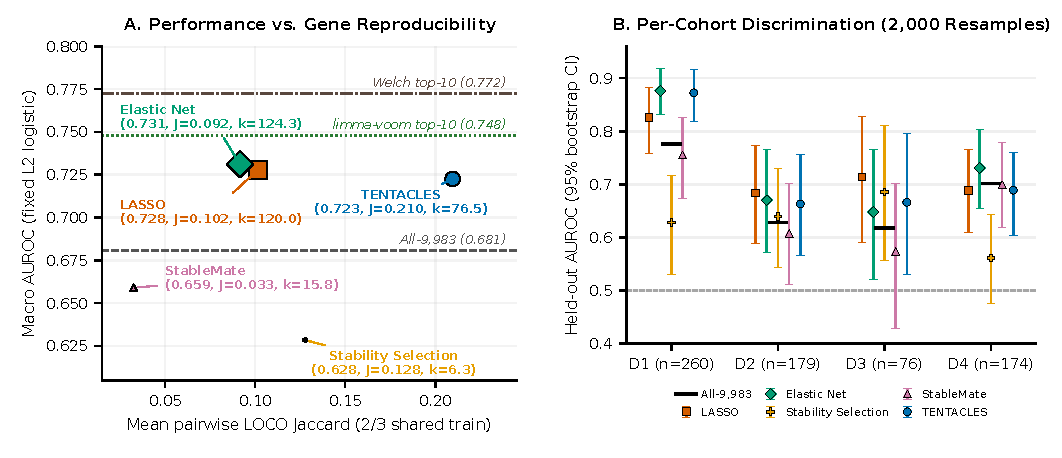
\includegraphics[width=\textwidth]{prediction_vs_agreement.pdf}
\caption{Prediction--reproducibility trade-off and per-cohort uncertainty. (A) Four-cohort mean held-out AUROC versus mean LOCO gene Jaccard (bubble area proportional to mean panel size $k$), anchored against All-9,983, \texttt{limma-voom} top-10 and Welch top-10 baselines. (B) Per-cohort AUROC with 2,000-resample stratified bootstrap 95\% CIs across D1--D4.}
\label{fig:tradeoff}
\end{figure*}

\begin{figure*}[!t]
\centering
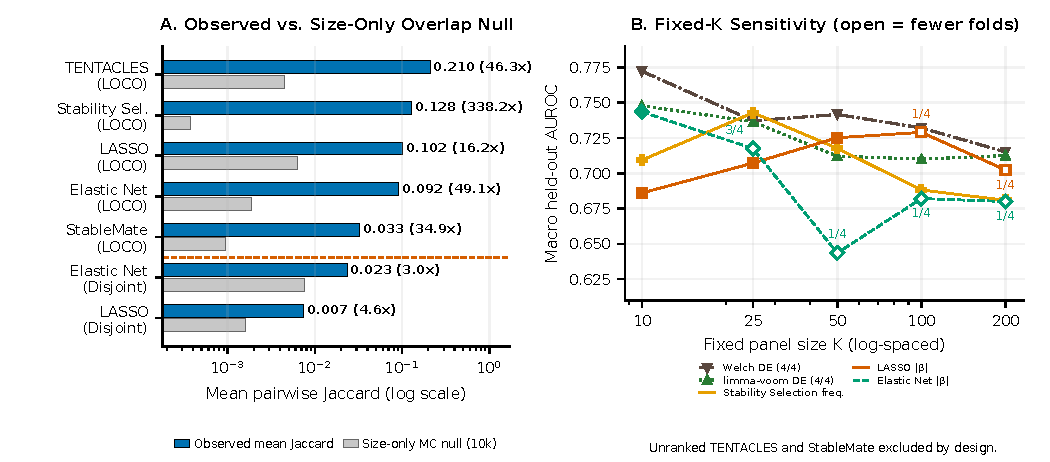
\includegraphics[width=\textwidth]{overlap_null_and_fixedK.pdf}
\caption{(A) Observed mean pairwise Jaccard versus size-only 10,000-draw Monte Carlo null across LOCO and disjoint single-cohort fits. (B) Fixed-$K$ sensitivity across continuously ranked methods; solid markers denote 4/4 evaluable folds, whereas open markers denote partial support ($<4/4$ folds) and must not be equated to four-fold means.}
\label{fig:overlap}
\end{figure*}

In patient-disjoint single-cohort fits, LASSO selected 27, 92, 9 and 31 genes for D1--D4, respectively, while Elastic Net selected 152, 198, 109 and 91 genes (Table~\ref{tab:independent_sizes}). All LASSO single-cohort fits selected fewer genes than the number of samples in the corresponding cohort. Across these disjoint cohorts, mean pairwise Jaccard was 0.007 for LASSO and 0.023 for Elastic Net, with no genes shared across all four independent fits.

\begin{table}[!t]
\caption{Gene panel sizes selected in disjoint single-cohort fits. These panels were not used for held-out prediction.}
\label{tab:independent_sizes}
\centering\scriptsize
\setlength{\tabcolsep}{2.4pt}
\resizebox{\columnwidth}{!}{\begin{tabular}{@{}lrrrrrl@{}}
\toprule
Selector / Solver & D1 & D2 & D3 & D4 & $\bar{J}$ (Obs/Null) & 4-Way\\
\midrule
LASSO (\texttt{liblinear}) & 27 & 92 & 9 & 31 & 0.007 / 0.002 & 0\\
Elastic Net (\texttt{glmnet}) & 152 & 198 & 109 & 91 & 0.023 / 0.008 & 0\\
\bottomrule
\end{tabular}}
\end{table}

\begin{table}[!t]
\caption{Fixed-$K$ panel-size sensitivity for continuously ranked methods. Partial-support means ($<4/4$ folds) are flagged explicitly and are not comparable to four-fold means.}
\label{tab:fixedk}
\centering\scriptsize
\setlength{\tabcolsep}{3.2pt}
\resizebox{\columnwidth}{!}{\begin{tabular}{@{}lrrlrr@{}}
\toprule
Method & $K$ & Folds & Cohorts & AUROC & BA\\
\midrule
LASSO & 10 / 25 / 50 & 4/4 & D1--D4 & 0.686 / 0.707 / 0.725 & 0.613 / 0.626 / 0.628\\
LASSO & 100 / 200 & 1/4 & D3 only & 0.729 / 0.702 & 0.605 / 0.587\\
Elastic Net & 10 & 4/4 & D1--D4 & 0.744 & 0.596\\
Elastic Net & 25 & 3/4 & D2--D4 & 0.717 & 0.620\\
Elastic Net & 50 / 100 / 200 & 1/4 & D3 only & 0.644 / 0.682 / 0.680 & 0.529 / 0.573 / 0.608\\
Stability Selection\ (rank) & 10 / 25 / 50 & 4/4 & D1--D4 & 0.709 / 0.743 / 0.718 & 0.613 / 0.598 / 0.588\\
Stability Selection\ (rank) & 100 / 200 & 4/4 & D1--D4 & 0.688 / 0.681 & 0.608 / 0.575\\
TENTACLES & 10--200 & 0/4 & None & \multicolumn{2}{c}{Unranked consensus (excluded)}\\
StableMate & 10--200 & 0/4 & None & \multicolumn{2}{c}{Unranked consensus (excluded)}\\
\bottomrule
\end{tabular}}
\end{table}

In fixed-$K$ sensitivity (Table~\ref{tab:fixedk}; Fig.~\ref{fig:overlap}B), Stability Selection (ranked frequency, evaluable on 4/4 folds across all $K$) rose from mean AUROC 0.628 ($\pi \ge 0.60$, mean 6.3 genes) to 0.709 at $K=10$ and 0.743 at $K=25$ before tapering to 0.681 at $K=200$. This shows that Stability Selection performance is sensitive to the number of ranked genes and is consistent with a small-panel handicap, although varying $K$ simultaneously alters gene membership, ranking truncation and downstream regularisation fit rather than isolating a single causal mechanism. LASSO was evaluable on 4/4 folds through $K=50$ and only 1/4 folds (D3, $n_{\mathrm{nonzero}}=219$) at $K=100,200$; Elastic Net was evaluable on 4/4 folds at $K=10$, 3/4 at $K=25$, and 1/4 (D3, $n_{\mathrm{nonzero}}=430$) at $K\ge 50$.

\subsection{Reactome pathway overlap and D3 QC sensitivity}
\label{sec:results_pathways}
Table~\ref{tab:results_pathways} summarises Reactome v98 enrichment for the TENTACLES, Stability Selection and StableMate panels. TENTACLES yielded 0, 11, 8 and 9 significant pathways across D1--D4, respectively (mean pathway Jaccard 0.256), including recurring interleukin-signalling and G-protein-coupled receptor pathways in D2--D4. Stability Selection and StableMate yielded no significant pathways in the assessed folds. Enrichment was not recalculated for the final LASSO or Elastic Net panels; their pathway results are therefore not reported or interpreted here.

\begin{table}[!t]
\caption{Reactome v98 enrichment ($q<0.05$) for gene panels with available final-analysis pathway results. A dash indicates that pathway agreement cannot be calculated when no significant pathways are present.}
\label{tab:results_pathways}
\centering\footnotesize
\setlength{\tabcolsep}{3.5pt}
\begin{tabular}{@{}lccc@{}}
\toprule
Method & D1/D2/D3/D4 & Folds & $\bar{J}$\\
\midrule
TENTACLES & 0/11/8/9 & 3/4 & 0.256\\
Stability Selection & 0/0/0/0 & 0/4 & ---\\
StableMate & 0/0/0/0 & 0/4 & ---\\
\bottomrule
\end{tabular}
\end{table}

Finally, excluding the seven source-flagged \texttt{qc=EXCLUDE} D3 samples in held-out test-only rescoring ($n=69$; Table~\ref{tab:s5}, Fig.~\ref{fig:s1}B) yielded small AUROC shifts for LASSO ($-0.005$), Elastic Net ($+0.002$), Stability Selection ($-0.015$) and StableMate ($-0.020$), and an increase of $+0.061$ for TENTACLES (AUROC $0.666 \to 0.726$; BA $+0.035$). Because D1, D2 and D4 were not retrained without these seven rows, these shifts quantify held-out test sensitivity rather than full-retraining sensitivity.

\section{Discussion}
\label{sec:discussion}
\subsection{Predictive transfer and gene-list consistency are distinct}
\label{sec:discussion_tradeoff}
This study tested whether feature-selection strategies that predict CD in an unseen cohort also return consistent gene lists. Under a fixed $L_2$ logistic classifier, Elastic Net (0.731), LASSO (0.728) and TENTACLES (0.723) achieved closely clustered mean AUROCs, while TENTACLES achieved the highest mean balanced accuracy (0.655). The highest-scoring selector changed across D1--D4, within-cohort 95\% bootstrap CIs overlapped broadly, and simple training-only differential-expression baselines (\texttt{limma-voom} and Welch $t$-test) matched or exceeded all complex selectors on descriptive mean AUROC. Even size-matched random panels achieved strong discrimination on D1 and D4. Consequently, raw cross-cohort AUROC alone does not justify complex selectors or establish statistical superiority across four dependent folds.

Gene agreement diverged markedly from prediction. TENTACLES achieved more than double the LOCO mean Jaccard of LASSO and Elastic Net (0.210 versus 0.102 and 0.092) on smaller panels (76.5 versus 120--124 genes). Fixed-$K$ sensitivity further confirmed that unequal panel sizes materially influence downstream AUROC. For example, mean AUROC for Stability Selection increased from 0.628 ($\pi \ge 0.60$) to 0.743 at $K=25$. This comparison does not isolate panel size as the sole causal factor. Correlated predictors substitute for one another across folds, and upstream tuning, preprocessing and support sizes all shape observed performance.

\subsection{What reproducibility can be inferred?}
\label{sec:discussion_reproducibility}
Because LOCO training pairs share two of three cohorts, their six pairwise Jaccard values quantify sensitivity to omitting one cohort rather than independent replication, and uniform Monte Carlo nulls serve strictly as size-only chance references rather than dependence-calibrated tests. In disjoint single-cohort fits, LASSO selected fewer genes than samples in every cohort. Elastic Net, which includes an $L_2$ penalty, can select more genes than samples. Mean pairwise Jaccard fell to 0.007 and 0.023, respectively, with zero four-way genes. Even disjoint cohorts may share annotation, upstream preprocessing or pipeline assumptions, so they are not a fully dependence-calibrated null model either.

\subsection{Pan-inflammatory signatures versus CD-specific biology and pathways}
\label{sec:discussion_pathway}
Because every cohort contrasts CD against \emph{Not IBD} controls without ulcerative colitis or non-IBD infectious colitis comparators, recurrently selected genes (\textit{NOS2}, \textit{MMP3}, \textit{CLDN18}, \textit{FFAR2}, \textit{PAQR5}, \textit{PML}) and recurring TENTACLES Reactome interleukin and GPCR pathways may reflect general intestinal mucosal inflammation and epithelial barrier disruption; CD specificity cannot be inferred. Distinguishing CD-specific biomarkers would require inflamed-control comparators (such as ulcerative colitis) and prospective clinical validation.

Pathway enrichment also remains conditional on panel size and annotation coverage. TENTACLES yielded significant terms in D2--D4 (and none in D1), whereas Stability Selection and StableMate produced zero significant pathways on their 4--20-gene panels. Pathway enrichment was not repeated on the final LASSO and Elastic Net panels, so their pathway-level reproducibility cannot be inferred from this analysis.

\subsection{Cohort composition and implementation limitations}
\label{sec:discussion_limits}
Four limitations bound interpretation. First, the four analytical cohorts combine six BioProjects differing in CD prevalence, biopsy site (with D4 tissue site missing), library depth and control source (including colorectal-cancer surgical tissue in D3); descriptive PCA reflects cohort structure without separating technical from biological variation. Second, D1--D3 arrived pre-filtered to 10,061 genes versus 41,257 in D4; without raw FASTQ reprocessing, the magnitude and potential differential impact of inherited upstream filtering remain unknown. Third, our D3 $n=69$ QC-exclusion analysis is strictly test-only rescoring rather than full cross-cohort retraining. Fourth, post-review work refitted LASSO and Elastic Net and added reference baselines, overlap nulls and fixed-$K$ analyses. TENTACLES, StableMate and Stability Selection use existing panels and saved results with controlled-classifier checks and updated uncertainty (Table~\ref{tab:s6}). TENTACLES native models were not retrained for this revision; prior learner-level warnings remain unresolved.

\subsection{Implications}
\label{sec:discussion_implications}
Transcriptomic benchmark reports should pair cohort-specific held-out metrics and uncertainty intervals with simple differential-expression and random-panel baselines, size-aware overlap references and clear model specifications and convergence checks, rather than reporting a single mean accuracy or consensus gene list. Within this four-cohort benchmark, the evidence supports an empirical comparison of candidate selectors, not clinically validated CD-specific biomarkers.

\section{Conclusion}
\label{sec:conclusion}
Across 689 intestinal RNA-seq samples, five feature-selection strategies and simple reference baselines demonstrated that cross-cohort predictive discrimination and gene-signature reproducibility are weakly coupled. Simple univariate differential expression matched complex selectors on descriptive mean AUROC, and ensemble consensus (TENTACLES) achieved the highest LOCO gene overlap without guaranteeing disjoint-cohort stability or CD-specific clinical validity. Predictive transfer, selection consistency and biological specificity must therefore be evaluated and reported as distinct outcomes.

\section*{Code and Data Availability}
The public project repository at \url{https://github.com/abbaselhajj/CMPS355-Transcriptomic-Feature-Selection} hosts the benchmark codebase, notebooks, methodological documentation, and the post-review results in the versioned revision directory. The complete LaTeX source, figures, and supplementary tables accompany this manuscript. The analysed RNA-seq datasets are identified by BioProject accession in Table~\ref{tab:cohorts} and described in the cited studies. No new patient data were collected.

\section*{Acknowledgment}
We thank Prof.\ Rida Assaf for research guidance and the peer reviewers for their constructive feedback. AI-assisted tools contributed to scripting, numerical checks and language editing; responsibility for the study design, data analysis and conclusions remains with the authors.

\bibliographystyle{IEEEtran}
\bibliography{references}
\clearpage
\onecolumn
\appendix
\section*{Supplementary Materials (Tables S1--S6 and Figure S1)}
\renewcommand{\thetable}{S\arabic{table}}
\setcounter{table}{0}
\renewcommand{\thefigure}{S\arabic{figure}}
\setcounter{figure}{0}
% Unique PDF anchors after restarting supplementary figure/table numbering.
\renewcommand{\theHfigure}{supp.\arabic{figure}}
\renewcommand{\theHtable}{supp.\arabic{table}}

\begin{figure}[!htbp]
\centering
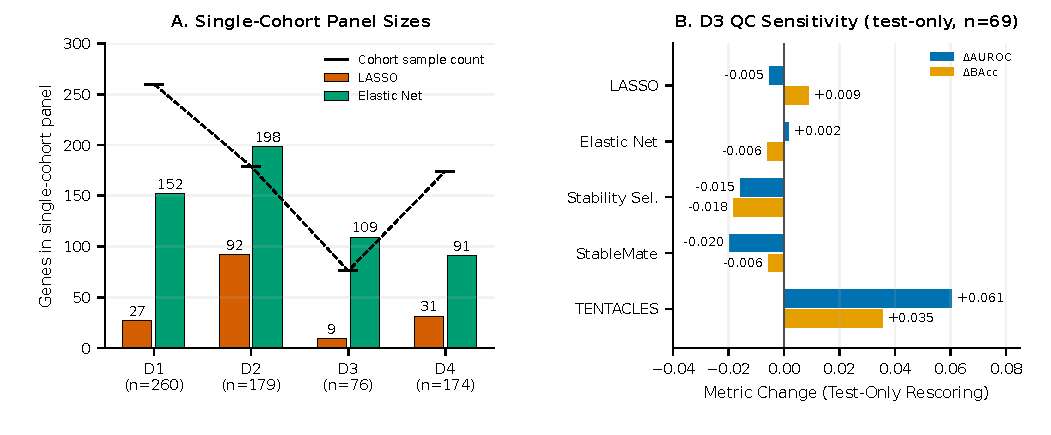
\includegraphics[width=\textwidth]{panel_sizes_and_d3_qc_sensitivity.pdf}
\caption{(A) Single-cohort LASSO and Elastic Net panel sizes relative to cohort sample counts, illustrating model sparsity. (B) Held-out D3 QC sensitivity: test-only rescoring excluding the seven source-flagged \texttt{qc=EXCLUDE} samples ($n=69$, training folds unchanged).}
\label{fig:s1}
\end{figure}

\begin{table}[!htbp]
\centering
\caption{Complete Per-Cohort Controlled-Classifier Metrics and 2,000-Resample Stratified Bootstrap 95\% CIs Across All Five Primary Methods}
\label{tab:s1}
\footnotesize
\setlength{\tabcolsep}{3.5pt}
\renewcommand{\arraystretch}{1.12}
\begin{tabular}{@{}lllrrrrrrrr@{}}
\toprule
Method & Coh. & $n$ (CD/NI) & AUROC [95\% CI] & BA [95\% CI] & AUPRC & Sens & Spec & Prec & F1 & Brier \\
\midrule
LASSO & D1 & 260 (218/42) & 0.8257 [0.7586, 0.8815] & 0.6007 [0.5389, 0.6694] & 0.9586 & 0.9633 & 0.2381 & 0.8678 & 0.9130 & 0.1385 \\
LASSO & D2 & 179 (134/45) & 0.6837 [0.5877, 0.7728] & 0.6349 [0.5608, 0.7017] & 0.8442 & 0.4254 & 0.8444 & 0.8906 & 0.5758 & 0.4087 \\
LASSO & D3 & 76 (34/42) & 0.7136 [0.5903, 0.8270] & 0.5987 [0.5133, 0.6821] & 0.7016 & 0.9118 & 0.2857 & 0.5082 & 0.6526 & 0.3882 \\
LASSO & D4 & 174 (109/65) & 0.6884 [0.6096, 0.7651] & 0.6445 [0.5708, 0.7152] & 0.7938 & 0.5505 & 0.7385 & 0.7792 & 0.6452 & 0.3026 \\
\midrule
Elastic Net & D1 & 260 (218/42) & 0.8760 [0.8307, 0.9183] & 0.4977 [0.4931, 0.5000] & 0.9755 & 0.9954 & 0.0000 & 0.8378 & 0.9099 & 0.1123 \\
Elastic Net & D2 & 179 (134/45) & 0.6700 [0.5716, 0.7647] & 0.5939 [0.5231, 0.6608] & 0.8395 & 0.3657 & 0.8222 & 0.8596 & 0.5131 & 0.4058 \\
Elastic Net & D3 & 76 (34/42) & 0.6478 [0.5203, 0.7661] & 0.5931 [0.4958, 0.6849] & 0.5841 & 0.8529 & 0.3333 & 0.5088 & 0.6374 & 0.3920 \\
Elastic Net & D4 & 174 (109/65) & 0.7307 [0.6539, 0.8027] & 0.6483 [0.6024, 0.6941] & 0.8503 & 0.3119 & 0.9846 & 0.9714 & 0.4722 & 0.3399 \\
\midrule
TENTACLES & D1 & 260 (218/42) & 0.8722 [0.8186, 0.9162] & 0.7911 [0.7155, 0.8621] & 0.9739 & 0.8440 & 0.7381 & 0.9436 & 0.8910 & 0.1253 \\
TENTACLES & D2 & 179 (134/45) & 0.6630 [0.5650, 0.7564] & 0.5845 [0.5103, 0.6624] & 0.8478 & 0.8134 & 0.3556 & 0.7899 & 0.8015 & 0.2232 \\
TENTACLES & D3 & 76 (34/42) & 0.6660 [0.5294, 0.7962] & 0.6275 [0.5119, 0.7339] & 0.7375 & 0.5882 & 0.6667 & 0.5882 & 0.5882 & 0.2948 \\
TENTACLES & D4 & 174 (109/65) & 0.6889 [0.6041, 0.7602] & 0.6172 [0.5512, 0.6770] & 0.8116 & 0.4037 & 0.8308 & 0.8000 & 0.5366 & 0.3002 \\
\midrule
StableMate & D1 & 260 (218/42) & 0.7555 [0.6736, 0.8267] & 0.7310 [0.6536, 0.8011] & 0.9292 & 0.7477 & 0.7143 & 0.9314 & 0.8295 & 0.1890 \\
StableMate & D2 & 179 (134/45) & 0.6078 [0.5114, 0.7017] & 0.5502 [0.4649, 0.6317] & 0.8250 & 0.5672 & 0.5333 & 0.7835 & 0.6580 & 0.2794 \\
StableMate & D3 & 76 (34/42) & 0.5735 [0.4293, 0.7024] & 0.4748 [0.3774, 0.5701] & 0.6573 & 0.7353 & 0.2143 & 0.4310 & 0.5435 & 0.4282 \\
StableMate & D4 & 174 (109/65) & 0.6994 [0.6178, 0.7787] & 0.6357 [0.5745, 0.6955] & 0.7910 & 0.3945 & 0.8769 & 0.8431 & 0.5375 & 0.3444 \\
\midrule
Stability Selection\ (0.60) & D1 & 260 (218/42) & 0.6278 [0.5306, 0.7174] & 0.5963 [0.5116, 0.6746] & 0.8879 & 0.6927 & 0.5000 & 0.8779 & 0.7744 & 0.2120 \\
Stability Selection\ (0.60) & D2 & 179 (134/45) & 0.6391 [0.5439, 0.7290] & 0.6129 [0.5347, 0.6872] & 0.8337 & 0.4701 & 0.7556 & 0.8514 & 0.6058 & 0.3264 \\
Stability Selection\ (0.60) & D3 & 76 (34/42) & 0.6856 [0.5574, 0.8109] & 0.5322 [0.4173, 0.6443] & 0.7394 & 0.5882 & 0.4762 & 0.4762 & 0.5263 & 0.2510 \\
Stability Selection\ (0.60) & D4 & 174 (109/65) & 0.5612 [0.4754, 0.6433] & 0.5097 [0.4545, 0.5696] & 0.7279 & 0.8349 & 0.1846 & 0.6319 & 0.7194 & 0.2438 \\
\bottomrule
\end{tabular}
\end{table}

\clearpage
\begin{table}[!htbp]
\centering
\caption{Reference Baselines Across All $K$ (4-Fold Macro; Sample SD, $n-1$ Denominator; Train-Eligible Uses $\mathrm{CPM}>1$ in $\ge 10\%$ of Training Samples)}
\label{tab:s2}
\footnotesize
\renewcommand{\arraystretch}{1.12}
\begin{tabular}{@{}lrrrrrr@{}}
\toprule
Baseline & $K$ & Macro AUROC (SD) & Macro BA (SD) & Macro AUPRC & Macro F1 & Macro Brier \\
\midrule
All-9,983 Shared Genes & 9,983 & 0.6808 (0.0734) & 0.5721 (0.0349) & 0.7752 & 0.6592 & 0.3362 \\
Train-Eligible ($\ge 10\%$ train) & 8,337--8,438 & 0.6733 (0.1300) & 0.5915 (0.0758) & 0.7639 & 0.6243 & 0.3713 \\
\texttt{limma-voom} DE & 10 & 0.7478 (0.1008) & 0.6310 (0.0944) & 0.8559 & 0.7225 & 0.2155 \\
\texttt{limma-voom} DE & 25 & 0.7365 (0.1072) & 0.6217 (0.0863) & 0.8317 & 0.6895 & 0.2314 \\
\texttt{limma-voom} DE & 50 & 0.7121 (0.0752) & 0.6280 (0.0219) & 0.8284 & 0.7021 & 0.2313 \\
\texttt{limma-voom} DE & 100 & 0.7100 (0.1175) & 0.6485 (0.1061) & 0.8141 & 0.7047 & 0.2356 \\
\texttt{limma-voom} DE & 200 & 0.7126 (0.0896) & 0.6414 (0.1129) & 0.8063 & 0.7778 & 0.2197 \\
Welch $t$-test DE & 10 & 0.7723 (0.0808) & 0.6007 (0.0808) & 0.8667 & 0.6248 & 0.2545 \\
Welch $t$-test DE & 25 & 0.7372 (0.0799) & 0.6049 (0.0523) & 0.8290 & 0.6666 & 0.2334 \\
Welch $t$-test DE & 50 & 0.7417 (0.0584) & 0.6566 (0.0461) & 0.8295 & 0.6639 & 0.2403 \\
Welch $t$-test DE & 100 & 0.7321 (0.0828) & 0.6601 (0.0636) & 0.8421 & 0.7224 & 0.2280 \\
Welch $t$-test DE & 200 & 0.7150 (0.1043) & 0.6556 (0.0815) & 0.8304 & 0.7692 & 0.2263 \\
\bottomrule
\end{tabular}
\end{table}

\begin{table}[!htbp]
\centering
\caption{Size-Matched Random-Panel Baselines ($B=100$ Draws per Cohort; 5th--95th Percentiles; Descriptive Within-Cohort $p_{\mathrm{emp}}$ Minimum Resolution $= 1/101 = 0.0099$)}
\label{tab:s3}
\footnotesize
\setlength{\tabcolsep}{3.8pt}
\renewcommand{\arraystretch}{1.10}
\begin{tabular}{@{}llrrrrrrrr@{}}
\toprule
Comparator & Coh. & $K$ & Obs AUROC & Null Mean & Null [5th, 95th] & $p_{\mathrm{emp}}$ (AUROC) & Obs BA & Null BA & $p_{\mathrm{emp}}$ (BA) \\
\midrule
LASSO & D1 & 94 & 0.8257 & 0.7964 & [0.7047, 0.8599] & 0.3267 & 0.6007 & 0.6473 & 0.6931 \\
LASSO & D2 & 77 & 0.6837 & 0.6161 & [0.5582, 0.6800] & 0.0594 & 0.6349 & 0.5714 & 0.0495 \\
LASSO & D3 & 219 & 0.7136 & 0.6406 & [0.5315, 0.7529] & 0.1683 & 0.5987 & 0.5564 & 0.2376 \\
LASSO & D4 & 90 & 0.6884 & 0.6829 & [0.5997, 0.7803] & 0.4752 & 0.6445 & 0.6249 & 0.3465 \\
\midrule
Elastic Net & D1 & 11 & 0.8760 & 0.6336 & [0.3879, 0.8098] & 0.0099 & 0.4977 & 0.5412 & 0.6733 \\
Elastic Net & D2 & 28 & 0.6700 & 0.6002 & [0.5388, 0.6553] & 0.0198 & 0.5939 & 0.5627 & 0.1782 \\
Elastic Net & D3 & 430 & 0.6478 & 0.6001 & [0.4667, 0.7086] & 0.3267 & 0.5931 & 0.5365 & 0.1584 \\
Elastic Net & D4 & 28 & 0.7307 & 0.6814 & [0.5461, 0.7850] & 0.2673 & 0.6483 & 0.6242 & 0.3861 \\
\midrule
TENTACLES & D1 & 73 & 0.8722 & 0.7937 & [0.6992, 0.8718] & 0.0594 & 0.7911 & 0.6241 & 0.0396 \\
TENTACLES & D2 & 91 & 0.6630 & 0.6182 & [0.5518, 0.6834] & 0.1386 & 0.5845 & 0.5773 & 0.4356 \\
TENTACLES & D3 & 81 & 0.6660 & 0.6645 & [0.5360, 0.7809] & 0.5446 & 0.6275 & 0.5703 & 0.1782 \\
TENTACLES & D4 & 61 & 0.6889 & 0.6848 & [0.5548, 0.7845] & 0.5743 & 0.6172 & 0.6228 & 0.6139 \\
\midrule
StableMate & D1 & 20 & 0.7555 & 0.7179 & [0.5069, 0.8544] & 0.3663 & 0.7310 & 0.5548 & 0.0396 \\
StableMate & D2 & 14 & 0.6078 & 0.5880 & [0.5027, 0.6661] & 0.3663 & 0.5502 & 0.5522 & 0.5248 \\
StableMate & D3 & 14 & 0.5735 & 0.6373 & [0.4731, 0.7686] & 0.7426 & 0.4748 & 0.5821 & 0.9604 \\
StableMate & D4 & 15 & 0.6994 & 0.6631 & [0.5169, 0.7776] & 0.3663 & 0.6357 & 0.6016 & 0.2871 \\
\midrule
Stability Selection\ (0.60) & D1 & 4 & 0.6278 & 0.5619 & [0.2846, 0.8253] & 0.3663 & 0.5963 & 0.5294 & 0.1782 \\
Stability Selection\ (0.60) & D2 & 9 & 0.6391 & 0.5658 & [0.4828, 0.6508] & 0.1089 & 0.6129 & 0.5402 & 0.0396 \\
Stability Selection\ (0.60) & D3 & 7 & 0.6856 & 0.6474 & [0.4919, 0.7857] & 0.3960 & 0.5322 & 0.5809 & 0.6733 \\
Stability Selection\ (0.60) & D4 & 5 & 0.5612 & 0.6040 & [0.4229, 0.7364] & 0.6832 & 0.5097 & 0.5651 & 0.7426 \\
\bottomrule
\end{tabular}
\end{table}

\clearpage
\begin{table}[!htbp]
\centering
\caption{Differing-Universe Pairwise and Four-Way Overlap Nulls (10,000 Monte Carlo Draws per Comparison)}
\label{tab:s4}
\footnotesize
\setlength{\tabcolsep}{3.2pt}
\renewcommand{\arraystretch}{1.12}
\begin{tabular}{@{}llrrrrrrl@{}}
\toprule
Method & Scope & Obs $\bar{J}$ & Null $\bar{J}$ & Ratio & Obs OC & 4-Way & Exact Exp & 4-Way Genes \\
\midrule
TENTACLES & LOCO (size-only) & 0.2097 & 0.0045 & 46.3$\times$ & 0.3829 & 6 & $5.44\times 10^{-5}$ & CLDN18, FFAR2, MMP3, NOS2, PAQR5, PML \\
Stability Selection\ (0.60) & LOCO (size-only) & 0.1278 & 0.0004 & 338.2$\times$ & 0.2726 & 0 & $2.09\times 10^{-9}$ & N/A \\
LASSO & LOCO (size-only) & 0.1016 & 0.0063 & 16.2$\times$ & 0.2563 & 2 & $2.36\times 10^{-4}$ & CLIC6, ZNF727 \\
Elastic Net & LOCO (size-only) & 0.0916 & 0.0019 & 49.1$\times$ & 0.2495 & 0 & $6.14\times 10^{-6}$ & N/A \\
StableMate & LOCO (size-only) & 0.0326 & 0.0009 & 34.9$\times$ & 0.0690 & 0 & $9.74\times 10^{-8}$ & N/A \\
Elastic Net (Disjoint) & Disjoint (0 shared) & 0.0233 & 0.0077 & 3.0$\times$ & 0.0618 & 0 & $4.92\times 10^{-4}$ & N/A \\
LASSO (Disjoint) & Disjoint (0 shared) & 0.0073 & 0.0016 & 4.6$\times$ & 0.0354 & 0 & $1.14\times 10^{-6}$ & N/A \\
\bottomrule
\end{tabular}
\end{table}

\begin{table}[!htbp]
\centering
\caption{D3 Held-Out QC Sensitivity Excluding Exact 7 \texttt{qc=EXCLUDE} Samples (Test-Only Rescoring, $n=69$; Training Folds Unchanged)}
\label{tab:s5}
\footnotesize
\setlength{\tabcolsep}{4.0pt}
\renewcommand{\arraystretch}{1.12}
\begin{tabular}{@{}lrrrrrrrrr@{}}
\toprule
Method & AUROC (76) & AUROC (69) & $\Delta$AUROC & BA (76) & BA (69) & $\Delta$BA & AUPRC & F1 & Brier \\
\midrule
LASSO & 0.7136 & 0.7085 & $-0.0050$ & 0.5987 & 0.6077 & $+0.0090$ & 0.6588 & 0.6512 & 0.3845 \\
Elastic Net & 0.6478 & 0.6496 & $+0.0018$ & 0.5931 & 0.5872 & $-0.0060$ & 0.5688 & 0.6265 & 0.4024 \\
Stability Selection (0.60) & 0.6856 & 0.6701 & $-0.0155$ & 0.5322 & 0.5141 & $-0.0181$ & 0.7161 & 0.5000 & 0.2564 \\
StableMate & 0.5735 & 0.5538 & $-0.0197$ & 0.4748 & 0.4692 & $-0.0056$ & 0.6325 & 0.5301 & 0.4391 \\
TENTACLES & 0.6660 & 0.7265 & $+0.0605$ & 0.6275 & 0.6628 & $+0.0354$ & 0.7750 & 0.6230 & 0.2513 \\
\bottomrule
\end{tabular}
\end{table}

\begin{table}[!htbp]
\centering
\caption{Computational provenance of the analyses reported in this study, distinguishing newly executed model fits from controlled downstream evaluation of existing gene panels.}
\label{tab:s6}
\footnotesize
\renewcommand{\arraystretch}{1.15}
\begin{tabularx}{\textwidth}{@{}p{3.2cm}XX@{}}
\toprule
Analysis & Execution basis & Implementation scope\\
\midrule
Input alignment & Reconstructed from source count matrices and R metadata & Sample identifiers and class labels aligned without modifying counts\\
LASSO and Elastic Net & Refitted on LOCO and single-cohort training splits & \texttt{liblinear} ($\mathrm{tol}=10^{-6}$) and \texttt{glmnet} ($\mathrm{thresh}=10^{-12}$) with KKT optimality checks\\
TENTACLES & Existing pre-review CD-positive nine-learner consensus panels and predictions & 6/9 primary and 5/9 sensitivity retained; downstream results checked and intervals updated; native training not repeated\\
StableMate and Stability Selection & Existing selected panels evaluated with the common downstream classifier & Downstream $L_2$ logistic fits and bootstrap intervals computed; method-native training not repeated\\
Simple reference baselines & Computed under identical LOCO splits and downstream classifier & All-9,983, train-eligible, \texttt{limma-voom}, Welch DE, and $B=100$ random panels\\
Overlap and fixed-$K$ analyses & Computed over fold-specific eligible gene universes & Exact expectations, 10,000-draw Monte Carlo nulls, and ranked fixed-$K$ evaluations\\
D3 QC sensitivity & New held-out-only rescoring of existing D3 predictions & Seven source-flagged samples excluded ($n=69$); no retraining of any fold\\
\bottomrule
\end{tabularx}
\end{table}

\end{document}
